\chapter{Generalized Bulletproofs e a prova de relações algébricas}
\label{chapter:generalized-bulletproofs}
\hypertarget{excerto.generalizadas.inicio}{}
\index{generalized bulletproofs@Generalized Bulletproofs}
\index{gbp@GBP|see{Generalized Bulletproofs}}

Suponhamos que o provador publicou dois compromissos. O primeiro guarda
dois números, o segundo guarda um só. Quer agora provar que o número
guardado no segundo é a soma dos quadrados dos outros dois. O verificador
tem diante de si dois pontos da curva. Pode somá-los, multiplicá-los por
escalares e comparar o resultado com outro ponto. Como há-de reconhecer,
nessas operações públicas, os dois quadrados que só o provador pode calcular?
Tomemos \(3^2+4^2=25\). Alice conhece o três e o quatro que
abrem o primeiro compromisso, bem como o vinte e cinco que abre o
segundo. Bob terá de reconhecer duas multiplicações, a soma dos
resultados e a ligação destes três números aos compromissos que recebeu.

Em bLSAG já encontrámos uma situação aparentada. O verificador multiplica
a chave candidata e a imagem de chave pelo mesmo desafio e usa a mesma
resposta em duas contas.
Na posição do signatário, a substituição da resposta faz reaparecer os
dois compromissos da ronda. Uma única testemunha explica ambas as contas.
Com várias testemunhas, a escolha dos multiplicadores exige outro cuidado.
Em CLSAG, cada segredo entra numa combinação definida pelo anel. Numa prova
de intervalo, há que distinguir as posições dos algarismos e os montantes a
que pertencem. Num circuito, há ainda que reconhecer o mesmo valor quando
sai de uma porta e entra noutra. Sigamos esses pesos desde a assinatura
de uma entrada até à prova sobre os dois compromissos.

\section{Uma resposta para as duas testemunhas de CLSAG}
\label{sec:gbp-pesos-clsag}
\index{clsag@CLSAG!pesos de agregacao@pesos de agregação}

O dono de uma saída conhece dois números de natureza bem diversa. Um
autoriza a despesa. O outro permite mostrar que a entrada conserva o
montante da saída que se gasta. Recordemos a coluna verdadeira do anel
de CLSAG, com o índice secreto \(\pi\) da Secção~\ref{sec:CLSAG}.
Se \(P_\pi=pG\) é a chave de uso único, \(C_\pi^{\mathrm{nz}}=\gamma G+vH\)
é o compromisso da saída e \(C_{\mathrm{off}}=\gamma'G+vH\) é a
pseudo-saída, a subtracção cancela o montante. Ficam as duas relações
\[
 P_\pi=pG,\qquad
 C_\pi^{\mathrm{nz}}-C_{\mathrm{off}}=(\gamma-\gamma')G=zG .
\]
A mesma posição \(\pi\) tem de servir para ambas. Uma resposta de
bLSAG, porém, usa um só escalar. Como hão-de caber nessa resposta a
chave \(p\) e a diferença de máscaras \(z\)?

Tomemos dois coeficientes \(\mu_P,\mu_C\) e multipliquemos a primeira
igualdade por \(\mu_P\) e a segunda por \(\mu_C\). Somando, o signatário
obtém o escalar \(w_\pi=\mu_Pp+\mu_Cz\). O verificador pode fazer a
mesma conta do lado dos pontos, para \emph{todas} as colunas, e obter
\[
 W_i=\mu_PP_i+\mu_C(C_i^{\mathrm{nz}}-C_{\mathrm{off}}).
\]
Numa delas vale \(W_\pi=w_\pi G\). Falta o segundo ponto que dá a
bLSAG a sua propriedade de ligação. Ponhamos \(J_i=\mathcal H_p(P_i)\).
As imagens \(I=pJ_\pi\) e \(D=zJ_\pi\) têm ambas a base \(J_\pi\).
Por isso, os mesmos pesos dão publicamente
\[
 \widetilde W=\mu_PI+\mu_CD=w_\pi J_\pi .
\]
A igualdade dos pesos nas duas contas tem uma consequência que o leitor
pode seguir até ao fecho do anel. Recebido o desafio \(c_\pi\), o
signatário escreve \(r_\pi=\alpha-c_\pi w_\pi\). O verificador
reconstitui os pontos
\[
 r_\pi G+c_\pi W_\pi=\alpha G,\qquad
 r_\pi J_\pi+c_\pi\widetilde W=\alpha J_\pi.
\]
O mesmo \(r_\pi\) restitui, nas duas bases, o compromisso que iniciou
a volta. O verificador refaz a volta a partir do desafio publicado,
empregando \(W_i,J_i\) próprios de cada posição, e compara o desafio
a que chegou com aquele de que partiu. Para reconhecer uma segunda
despesa, compara a imagem \(I\), que depende unicamente da chave de
uso único. As equações de pontos desta passagem são as do subgrupo
de ordem prima \(l\).

Há uma escolha essencial por trás desta conta tão simples. Quem determina
a proporção em que entram \(p\) e \(z\)? Os pesos provêm de dois domínios
de hash distintos, aplicados aos mesmos dados públicos. Estes compreendem
o anel ordenado de chaves e compromissos, a imagem \(I\), a representação
de \(D\) transmitida na assinatura e a pseudo-saída. Assim, qualquer dos
participantes pode refazer a escolha. Se se alterar um dos compromissos,
há que calcular de novo \emph{ambos} os pesos, inclusive aquele que
multiplica as chaves. E cada peso vale em todo o anel, pois distingue
as duas relações que se pretendem reunir. São os desafios \(c_i\) que
mudam ao passar de uma coluna à seguinte~\cite{MRL-0011-CLSAG}.

Convém medir exactamente o alcance de uma combinação destas. Fixadas
duas diferenças de escalares \((e_P,e_C)\ne(0,0)\), a combinação
perde-as quando \(\mu_Pe_P+\mu_Ce_C=0\). Se \(e_C\ne0\), uma vez
escolhido \(\mu_P\), há um único valor favorável de \(\mu_C\),
precisamente \(-\mu_Pe_P/e_C\). Com dois pesos uniformes independentes
em \(\mathbb F_l\), a probabilidade é \(1/l\). Para \(e_C=0\), a
equação exige \(\mu_P=0\) e a contagem é a mesma. Trata-se da conta
para erros fixados antes da escolha. Na assinatura, a possibilidade de
o adversário escolher chaves, consultar o hash e tentar de novo pertence
à análise criptográfica de CLSAG, com as suas hipóteses sobre a
agregação de chaves e os logaritmos discretos. O que o fecho de bLSAG
usa directamente é o escalar agregado. A garantia relativa às chaves
que participaram na sua formação vem dessa análise~\cite{MRL-0011-CLSAG}.

\section{Dos algarismos de um montante ao produto ponderado}
\label{sec:gbp-pesos-intervalo}
\index{bulletproofs@Bulletproofs!pesos das restricoes@pesos das restrições}
\index{bulletproofs+@Bulletproofs+!produto interno ponderado@produto interno ponderado}

Passemos agora da entrada à saída. O compromisso \(V=\gamma G+vH\)
esconde um montante, e a sua prova de intervalo certifica que há \(n\)
bits cuja soma, com os devidos pesos, é \(v\). Logo aqui surgem pesos
que todos conhecem de antemão. Para \(n=4\), os dígitos
\((0,1,1,0)\), começando pelas unidades, representam
\(0\cdot1+1\cdot2+1\cdot4+0\cdot8=6\). O número \(2^i\) dá ao
algarismo da posição \(i\) o seu valor em unidades. Os outros pesos da
prova respondem a uma pergunta diferente. Como poderá o verificador
testar a condição \emph{em cada posição}, se os algarismos lhe estão
vedados?

Na Bulletproof clássica, o provador fixa os vectores
\(\boldsymbol a_L,\boldsymbol a_R\) antes de receber o desafio \(y\).
Chamemos \(a_i,b_i\) às suas coordenadas. Queremos que \(a_ib_i=0\)
e \(a_i-b_i=1\) para todo o \(i\). Em conjunto, estas condições dão
\(a_i(a_i-1)=0\), cujas únicas soluções num corpo são \(0\) e \(1\).
Atribua-se, por exemplo,
uma diferença \(h\ne0\) à posição zero e \(-h\) à posição um. A
soma ponderada por \(1,y\) é \(h-hy\), e só desaparece quando \(y=1\).
Com \(n\) posições, a soma ponderada é um polinómio de grau até
\(n-1\). Esta é a razão de se poderem obter todos os pesos de posição
a partir de um único desafio.

É possível acompanhar na mesma conta os três requisitos da prova.
Chamemos \(A(Y), B(Y)\) aos polinómios dos desvios e \(D_v\) à
diferença de montante,
\[
 A(Y)=\sum_{i=0}^{n-1}a_ib_iY^i,\qquad
 B(Y)=\sum_{i=0}^{n-1}(a_i-b_i-1)Y^i,\qquad
 D_v=\sum_{i=0}^{n-1}2^ia_i-v .
\]
Os nomes \(A(Y),B(Y)\) designam aqui polinómios escalares. Com
\(y,z\) extraídos sucessivamente da transcrição, a diferença que nos interessa
é o escalar
\begin{equation}
 E(y,z)=A(y)+zB(y)+z^2D_v.
 \label{eq:gbp-bp-residuos}
\end{equation}
O expoente de \(y\) designa uma posição, e o expoente de \(z\) designa
uma espécie de condição. Se \(A=B=0\) como polinómios e \(D_v=0\),
a diferença é zero para todos os desafios. Se uma das condições falhar,
\(E(Y,Z)\) é um polinómio não nulo. Suponhamos os vectores e o montante
fixos, e os desafios uniformes e independentes em \(\mathbb F_l^*\).
Se um dos polinómios \(A,B\) for não nulo, a probabilidade de \(y\)
anular esse polinómio é no máximo \((n-1)/(l-1)\). Sempre que algum
coeficiente sobreviva, restam no máximo duas raízes para \(z\). Em
conjunto, estas duas ocasiões de coincidência têm probabilidade no
máximo \((n+1)/(l-1)\). Esta estimativa diz respeito precisamente à
redução das três condições, com uma só escolha dos desafios.

Como chega esta conta ao verificador? Multipliquemos os factores
\(a_i-z\) e \(y^i(b_i+z)+z^2\,2^i\) e somemos em \(i\). Os termos em
\(y^i\) dão \(a_ib_i+z(a_i-b_i)-z^2\), cada qual multiplicado
pela sua potência. Os termos com \(2^i\) dão \(z^2\sum_i2^ia_i-
z^3\sum_i2^i\). Separando o montante e a parte inteiramente pública,
obtém-se
\begin{align*}
 t_0
   &=\sum_i(a_i-z)\bigl[y^i(b_i+z)+z^2\,2^i\bigr]\\
   &=z^2v+\delta(y,z)+E(y,z),\\
 \delta(y,z)&=(z-z^2)\sum_i y^i-z^3\sum_i2^i .
\end{align*}
O erro da Equação~\eqref{eq:gbp-bp-residuos} é assim a diferença
exacta entre o termo constante do produto interno e o valor que o
compromisso permite conferir. Na prova honesta, a contribuição de
\(v\) entra no ponto público \(z^2V\), que leva consigo a contribuição
\(z^2\gamma\) da máscara. Somam-se a esse ponto o termo público
\(\delta(y,z)H\) e os compromissos \(xT_1+x^2T_2\) dos dois termos
de grau positivo. O desafio \(x\) vem depois de \(T_1,T_2\). O
verificador confere a igualdade com \(t(x)H+\tau_xG\), e o argumento
de produto interno liga \(t(x)\) aos mesmos vectores mascarados, como
nas Equações~\eqref{eq:bp-value-check} e~\eqref{eq:bp-public-ip-point}.
Quando há várias saídas, a saída \(j\), contando de zero, recebe o
peso \(z^{j+2}\) no lugar de \(z^2\). Os seus bits continuam a valer
\(1,2,4,\ldots\) dentro da própria saída~\cite{Bulletproofs_paper}.

Em Bulletproofs+ a ponderação acompanha o produto interno até ao seu
último termo~\cite{bulletproofs-plus-paper}. Com os índices a começar
em zero e \(n\) coordenadas no total, define-se
\[
 [\boldsymbol a,\boldsymbol b]_y
   =\sum_{i=0}^{n-1}y^{i+1}a_i b_i .
\]
Vejamos como se consegue que cada montante surja ainda com o seu
valor inteiro, embora cada posição tenha agora um peso diferente.
Se há \(N\) bits por saída, ponhamos
\(d_{jN+k}=z^{2(j+1)}2^k\), com \(0\le k<N\). Para duas saídas,
de dois bits cada, fica
\[
 \boldsymbol d=(z^2,2z^2,z^4,2z^4).
\]
Se os bits forem \((1,0,0,1)\), os montantes são \(1\) e \(2\).
O produto \(\sum_i a_id_i\) dá precisamente \(z^2+2z^4\).
Nas provas de intervalo de Monero, cada saída ocupa \(N=64\)
posições, e completa-se o número de saídas até uma potência de dois
com montantes e máscaras nulos.

O provador forma \(a'_i=a_i-z\) e
\(b'_i=b_i+z+d_i y^{n-i}\), como na
Equação~\eqref{eq:bpp-prime-vectors}. O expoente descendente em
\(b'_i\) tem uma razão aritmética. Ao tomar o produto ponderado,
\(y^{i+1}y^{n-i}=y^{n+1}\) em \emph{todas} as posições.
A contribuição do montante sai por isso da soma com um factor comum.
Para bits válidos, \((a_i-z)(b_i+z)=z-z^2\). Logo,
\begin{align*}
 [\boldsymbol a',\boldsymbol b']_y
 &= (z-z^2)\sum_i y^{i+1}
       +y^{n+1}\left(\sum_j z^{2(j+1)}v_j-z\sum_i d_i\right)\\
 &= \delta_+ + y^{n+1}\sum_j z^{2(j+1)}v_j,\\
 \delta_+&=(z-z^2)\sum_i y^{i+1}-z y^{n+1}\sum_i d_i .
\end{align*}
Voltando às duas saídas, cada bit entrou com o seu peso próprio no
teste de que era um bit, mas os dois montantes entraram no resultado
pelos pesos \(y^5 z^2\) e \(y^5 z^4\). O verificador pode já fazer
essa última combinação com os \emph{compromissos} dos montantes.

Mesmo com algarismos arbitrários, a expansão diz exactamente
o que falta para a igualdade. Ponha-se
\(D_j=\sum_{k=0}^{N-1}2^k a_{jN+k}-v_j\).
Subtraindo ao produto o valor esperado, resta
\[
 \sum_i y^{i+1}a_i b_i
 +z\sum_i y^{i+1}(a_i-b_i-1)
 +y^{n+1}\sum_j z^{2(j+1)}D_j .
\]
Vê-se por que se distinguem os montantes nesta prova. O termo
constante em \(z\) recolhe os produtos dos algarismos, o termo de
grau um recolhe as diferenças entre os dois vectores, e cada
montante tem um grau par próprio, começando em dois. Os termos de
grau ímpar que provêm de \(-z\sum_i d_i\) já entraram na correcção
pública \(\delta_+\). Se o segundo montante do exemplo valesse
três no compromisso e dois na decomposição, sobraria exactamente
\(-y^5z^4\). Para \(y,z\ne0\), esse desvio isolado é sempre visível.

Escrevamos todos os pontos seguintes na sua forma matemática, depois
da reposição do cofactor descrita na Secção~\ref{sec:bulletproof_plus}.
Seja \(A_0\) o compromisso inicial aos vectores de coordenadas
\(a_i,b_i\), com máscara \(\alpha\). O verificador constrói o ponto
\begin{align*}
 P={}&A_0-z\sum_iG_i+\sum_i(z+d_i y^{n-i})H_i\\
    &+y^{n+1}\sum_j z^{2(j+1)}C_j+\delta_+ H .
\end{align*}
As duas correcções vectoriais trocam \(a_i,b_i\) por \(a'_i,b'_i\).
A soma dos \(C_j=\gamma_jG+v_jH\) traz nos seus coeficientes de \(H\)
os montantes necessários. Nos de \(G\) traz as respectivas máscaras.
O provador conhece assim a abertura
\[
 P=\sum_i(a'_iG_i+b'_iH_i)
       +[\boldsymbol a',\boldsymbol b']_y H+\alpha'G,\qquad
 \alpha'=\alpha+y^{n+1}\sum_j z^{2(j+1)}\gamma_j.
\]
O ponto à esquerda provém de dados públicos. A abertura à direita
constitui a afirmação que resta provar.

Acompanhemos o peso de uma coordenada durante uma dobra. Se houver
\(2h\) coordenadas, a metade direita principia com \(y^{h+1}\), ao
passo que a primeira principiava com \(y\). Abreviemos os dois
vectores do passo corrente por \(a,b\), com metades \(a_L,a_R\) e
\(b_L,b_R\). O seu produto é a soma de
\([a_L,b_L]_y\) e \(y^h[a_R,b_R]_y\), usando produtos de comprimento
\(h\). Para o desafio não nulo \(u\) desta dobra tomam-se
\[
 a'=u a_L+u^{-1}y^h a_R,\qquad b'=u^{-1}b_L+u b_R .
\]
Multiplicando, reaparece o produto antigo, acrescido dos dois termos
cruzados \(u^2[a_L,b_R]_y\) e \(u^{-2}y^h[a_R,b_L]_y\).
Eis por que entram \(u^2\) e \(u^{-2}\) na actualização pública
\(P'=P+u^2L+u^{-2}R\). Os pontos \(L,R\) comprometeram previamente
os termos cruzados e as correspondentes combinações de geradores.
Nos geradores de \(a\) a dobra usa
\(u^{-1}\boldsymbol G_L+u y^{-h}\boldsymbol G_R\), e nos de \(b\)
usa \(u\boldsymbol H_L+u^{-1}\boldsymbol H_R\). Basta multiplicar os
factores da metade direita para reconhecer \((u^{-1}y^h)(u y^{-h})=1\).
Aquela metade conserva, portanto, tanto a sua abertura linear como o
seu lugar no produto ponderado.

Finda a última dobra, a afirmação que resta tem dois números secretos
\(a^\star,b^\star\) e um ponto público
\[
 P^\star=a^\star G^\star+b^\star H^\star+
             y a^\star b^\star H+\alpha^\star G.
\]
O provador enviou os compromissos finais \(A_1,B\) e respondeu ao
desafio \(e\) com \(r_1,s_1,d_1\), como nas
Equações~\eqref{eq:bpp-a1} a~\eqref{eq:bpp-d1}. Na mesma convenção
de pontos matemáticos, o verificador testa
\[
 B+eA_1+e^2P^\star
   =e r_1G^\star+e s_1H^\star+y r_1s_1H+d_1G .
\]
O coeficiente de \(H\) permite ler a igualdade de ponta a ponta.
Com \(r_1=r+ea^\star\) e \(s_1=s+eb^\star\), o produto \(y r_1s_1\)
tem termo constante \(yrs\) em \(B\), termo linear
\(ey(rb^\star+sa^\star)\) em \(eA_1\) e termo quadrático
\(e^2y a^\star b^\star\) em \(e^2P^\star\). O factor \(y\) da
primeira coordenada reaparece ainda na conta que decide a aceitação.

Resta distinguir uma escolha feita pelo próprio verificador, já de
posse das provas completas. Uma igualdade entre pontos equivale a
pedir que a diferença entre os membros dê a identidade \(\mathcal O\).
Se \(F_j\) for essa diferença na prova \(j\), o verificador pode
sortear pesos independentes \(w_j\) uniformes em \(\mathbb F_l^*\)
e testar \(\sum_j w_jF_j=\mathcal O\). Sempre que algum
\(F_k\ne\mathcal O\), fixar os restantes pesos deixa no máximo uma
escolha favorável para \(w_k\), porque \(F_k\) tem ordem \(l\). A
probabilidade de aceitar por cancelamento no lote é assim, no máximo,
\(1/(l-1)\). Na Bulletproof clássica há duas equações por prova e
podem sortear-se pesos distintos para ambas. Em Bulletproofs+ basta um
peso por prova. Estes pesos do lote multiplicam equações já formadas.
Os pesos \(y,z\), esses, foram necessários para \emph{formar} a
equação de cada prova.

As provas de intervalo dispõem da mesma conta em todas as posições,
\(a_i(a_i-1)=0\). Um circuito aritmético permite que o produto numa
posição seja a entrada da posição seguinte, que uma soma tenha valor
público, ou que um dos seus vectores esteja já fixado num compromisso
exterior. Para reunir tais condições há que saber, além da posição de
cada produto, com que coeficiente cada fio figura em cada equação.
É essa informação que os pesos vão transportar para o produto interno
das Generalized Bulletproofs.

\section{Calcular com números já comprometidos}
\label{sec:gbp-circuito}
\index{circuito aritmetico@circuito aritmético!aberturas vectoriais@aberturas vectoriais}

Voltemos aos dois compromissos. Num grupo de ordem prima \(p\), escrevamos
\[
  K=u g_1+w g_2+\eta h,\qquad V=v g+\gamma h .
\]
O provador conhece \(u,w,v\) e as duas máscaras. O verificador conhece
\(K,V\) e as bases públicas. Nesta notação do circuito, \(g\) recebe
o valor escalar e \(h\) recebe a máscara. O verificador quer uma prova de que \(u^2+w^2=v\), no
corpo de escalares \(\mathbb F_p\), com os três valores tomados das
aberturas daqueles pontos. Se \(u=3\), \(w=4\), a testemunha dá
\(v=25\). As igualdades seguintes explicam como se pode verificar a conta
mesmo quando os três valores permanecem ocultos.

Demos duas portas de multiplicação ao provador. Em cada porta ele põe
um operando esquerdo, um operando direito e um resultado. Com os valores
do exemplo, os vectores das três colunas são
\[
 \boldsymbol a_L=(3,4),\qquad \boldsymbol a_R=(3,4),\qquad
 \boldsymbol a_O=(9,16).
\]
A regra das portas é \(\boldsymbol a_L\circ\boldsymbol a_R=\boldsymbol a_O\).
Para que as portas executem precisamente o cálculo prometido, escrevemos
também as cinco ligações
\begin{equation}
 \begin{aligned}
  a_{L,1}-u&=0, & a_{R,1}-u&=0,\\
  a_{L,2}-w&=0, & a_{R,2}-w&=0,\\
  a_{O,1}+a_{O,2}&=v .
 \end{aligned}
 \label{eq:gbp-duas-portas}
\end{equation}
Assim se obriga a primeira porta a receber duas vezes o mesmo \(u\) de
\(K\), e a segunda a receber duas vezes o mesmo \(w\). A última linha
entrega a soma dos resultados ao valor de \(V\). Os cinco traços que
ligaríamos num desenho do circuito são cinco equações lineares.

A figura reúne estas cinco ligações. Cada caixa de multiplicação
recebe dois fios. O nome escrito em cada fio refere a posição
efectiva que lhe cabe na porta. A soma da direita é uma relação
linear nos resultados. O provador pode, por isso, descrevê-la
sem acrescentar uma terceira porta de multiplicação.
\begin{center}
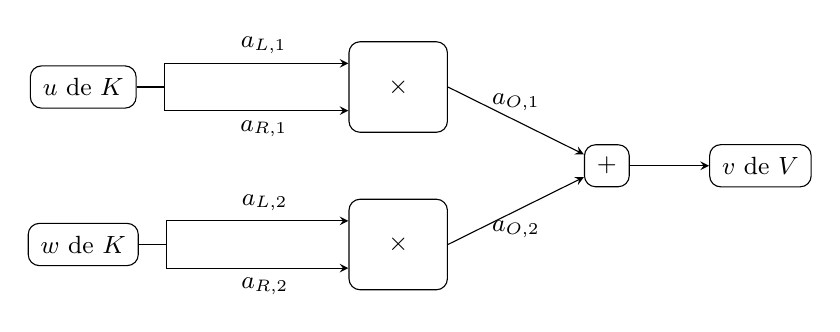
\begin{tikzpicture}[>=stealth,font=\small,
 block/.style={draw,rounded corners,align=center,inner sep=4.5pt}]
 \node[block] (u) at (-4.5,1) {\(u\) de \(K\)};
 \node[block] (w) at (-4.5,-1) {\(w\) de \(K\)};
 \node[block,minimum height=1.15cm,minimum width=1.25cm] (p) at (-.5,1) {\(\times\)};
 \node[block,minimum height=1.15cm,minimum width=1.25cm] (q) at (-.5,-1) {\(\times\)};
 \node[block] (sum) at (2.15,0) {\(+\)};
 \node[block] (v) at (4.1,0) {\(v\) de \(V\)};
 \draw[->] (u.east)--++(.35,0)|- ([yshift=3mm]p.west)
   node[pos=.77,above] {\(a_{L,1}\)};
 \draw[->] (u.east)--++(.35,0)|- ([yshift=-3mm]p.west)
   node[pos=.77,below] {\(a_{R,1}\)};
 \draw[->] (w.east)--++(.35,0)|- ([yshift=3mm]q.west)
   node[pos=.77,above] {\(a_{L,2}\)};
 \draw[->] (w.east)--++(.35,0)|- ([yshift=-3mm]q.west)
   node[pos=.77,below] {\(a_{R,2}\)};
 \draw[->] (p.east)--node[midway,above] {\(a_{O,1}\)} (sum);
 \draw[->] (q.east)--node[midway,below] {\(a_{O,2}\)} (sum);
 \draw[->] (sum)--(v);
\end{tikzpicture}
\end{center}

Retenhamos a disposição da figura e perguntemos o que terá de fixar
uma descrição pública deste circuito. O primeiro fio pode receber
qualquer elemento do corpo, mas a sua origem é a primeira coordenada
de \(K\). O segundo recebe a mesma coordenada e leva-a ao segundo operando da porta. O verificador
pode numerar os fios e indicar de antemão onde começa e onde acaba
cada um. Nesta descrição a posição de um valor é pública. O valor
que Alice escreverá nessa posição pertence à sua testemunha.

Tomemos por ordem os seis números das portas e os três números
comprometidos. Escrevamos o vector das suas posições como
\[
 \boldsymbol z_0=(a_{L,1},a_{L,2},a_{R,1},a_{R,2},
                      a_{O,1},a_{O,2},u,w,v)^\top .
\]
Esta letra com índice zero designa apenas as nove posições deste
quadro. As cinco linhas seguintes descrevem os fios. Uma entrada
\(1\) conserva o sinal da posição respectiva e uma entrada
\(-1\) subtrai-a. Os espaços em branco valem zero.
\[
\begin{array}{c|rr|rr|rr|rr|r}
 &a_{L,1}&a_{L,2}&a_{R,1}&a_{R,2}&a_{O,1}&a_{O,2}&u&w&v\\ \hline
 1&1&&&&&&-1&&\\
 2&&&1&&&&-1&&\\
 3&&1&&&&&&-1&\\
 4&&&&1&&&&-1&\\
 5&&&&&1&1&&&-1
\end{array}
\]
Designemos a matriz por \(M\). Para a testemunha dos quadrados,
o vector que ela multiplica é \((3,4,3,4,9,16,3,4,25)^\top\).
Ler o quadro na horizontal dá \(3-3,3-3,4-4,4-4,9+16-25\).
É essa a igualdade \(M\boldsymbol z_0=\boldsymbol0\). Já o
produto de cada porta lê-se na vertical entre posições
correspondentes dos três primeiros pares de colunas. Combinar as
descrições obriga o três a chegar a ambos os operandos da primeira
porta, o quatro a chegar a ambos os operandos da segunda e a soma
dos quadrados a terminar no compromisso escalar.

Há ainda outra leitura, particularmente económica para quem
verifica. Demos pesos \(q_1,\ldots,q_5\) às linhas e somemo-las.
Para saber que parte da combinação vem de \(u\), basta percorrer a
coluna de \(u\). Duas linhas lhe atribuíram \(-1\), pelo que lhe cabe o coeficiente \(-q_1-q_2\). A coordenada \(w\) recebe
\(-q_3-q_4\). Ao valor \(v\) chega só \(-q_5\), e ambos os
resultados das portas recebem \(+q_5\). Podemos ler de uma vez
a combinação inteira
\[
 \begin{aligned}
 &q_1a_{L,1}+q_3a_{L,2}
     +q_2a_{R,1}+q_4a_{R,2}
     +q_5(a_{O,1}+a_{O,2})\\
 &\hspace{18mm}-(q_1+q_2)u-(q_3+q_4)w-q_5v .
 \end{aligned}
\]
Substituir a testemunha honesta anula a expressão quaisquer que
sejam os pesos. O ponto de vista do verificador é o inverso.
Sendo-lhe ocultas as entradas do vector, ele prepara a combinação
por meio dos coeficientes das colunas. O que poderá calcular com
as bases públicas e os compromissos será justamente uma igualdade
que contenha essa combinação. A transposta da matriz irá aparecer
porque reúne, numa só operação, os pesos de todas as linhas por onde
passa cada coordenada.

Vejamos essa troca com números. Ponhamos
\((q_1,q_2,q_3,q_4,q_5)=(2,4,8,16,32)\). A combinação das linhas
atribui \(-6\) à primeira coordenada de \(K\) e \(-24\) à segunda.
Percorrendo as ligações com as aberturas \(u=3,w=4\), chegam
\(2\cdot3+8\cdot4=38\) pelo lado esquerdo das portas e
\(4\cdot3+16\cdot4=76\) pelo lado direito. A parcela de \(K\)
vale \(-6\cdot3-24\cdot4=-114\), que cancela exactamente
\(38+76\). Pelos resultados chegam \(32(9+16)=800\), e no valor
de \(V\) espera-os \(-32\cdot25=-800\). Pode fazer-se esta conta
nos inteiros e tomar o resultado no corpo de escalares. Para qualquer
número de portas, a cada ocorrência de uma
variável corresponde uma entrada na matriz, e os contributos de
todas as suas ocorrências juntam-se na coluna que lhe cabe.

Os compromissos exteriores dão a estas ligações uma consequência
observável. \(3^2+4^2\) e \(4^2+3^2\) dão ambos \(25\).
A declaração que conhece somente o resultado admite ambas as ordens
dos operandos. No compromisso \(K\), contudo, a primeira coordenada
multiplica \(g_1\) e a segunda multiplica \(g_2\). Mantida a
máscara, passar de \((3,4)\) para \((4,3)\) desloca o ponto por
\(g_1-g_2\). O circuito tem, por isso, uma razão para dar nome
próprio às duas posições, mesmo ao efectuar uma soma simétrica.
Está a demonstrar que a relação vale para os valores que entraram
naqueles lugares dos compromissos publicados.


A generalização consiste em poder designar, em qualquer destas equações,
a coordenada de um compromisso vectorial que já faz parte da declaração.
Fixemos uma dimensão \(m\), potência de dois, que comporte as portas
e os vectores comprometidos. Para \(s\) compromissos vectoriais e
\(r\) compromissos escalares a declaração de conhecimento admite
as aberturas
\begin{equation}
 \begin{aligned}
 K_k&=\langle\boldsymbol c_k,\boldsymbol g\rangle+
       \langle\boldsymbol d_k,\boldsymbol h\rangle+\eta_k h
       &&(1\leq k\leq s),\\
 V_j&=v_jg+\gamma_j h &&(1\leq j\leq r).
 \end{aligned}
 \label{eq:gbp-aberturas}
\end{equation}
As duas famílias vectoriais \(\boldsymbol g,\boldsymbol h\) têm
\(m\) bases cada uma. A segurança pressupõe que seja impraticável
encontrar uma relação de logaritmo discreto não trivial na família
completa, incluindo \(g,h\). O circuito refere as coordenadas
\(\boldsymbol c_k\). O vector \(\boldsymbol d_k\) também faz parte
da abertura cuja existência se demonstra. Quem forma \(K\) como acima
conhece a abertura com \(\boldsymbol d_1=\boldsymbol 0\). Se o mesmo
ponto tiver de corresponder a uma abertura já estabelecida noutra prova,
é a vinculação do compromisso que permite identificá-las. Subtrair duas
aberturas diferentes e conhecidas produziria precisamente uma relação
entre as bases. Esta distinção terá efeito quando o compromisso guardar
um ramo de uma árvore~\cite{generalized-bulletproofs-fixed,fcmp-composition-review}.

Sejam \(q\) as ligações lineares. Para as ler todas de uma vez,
disponhamos os seus coeficientes em matrizes públicas, uma linha por
ligação. A declaração completa exige as aberturas
\eqref{eq:gbp-aberturas} e as igualdades
\begin{equation}
 \begin{aligned}
  \boldsymbol a_L\circ\boldsymbol a_R&=\boldsymbol a_O,\\
  W_L\boldsymbol a_L+W_R\boldsymbol a_R+W_O\boldsymbol a_O
      +\sum_{k=1}^{s}W_k\boldsymbol c_k
     &=\boldsymbol b+W_V\boldsymbol v .
 \end{aligned}
 \label{eq:gbp-relacao}
\end{equation}
Aqui \(\boldsymbol b\) contém as \(q\) constantes. Cada matriz da
esquerda tem \(q\) linhas e \(m\) colunas. A matriz \(W_V\), à direita,
tem \(r\) colunas e supõe-se de posto \(r\). Esta condição permite
recuperar cada abertura escalar a partir de combinações bastantes das
linhas. No nosso exemplo \(r=1\), \(\boldsymbol b=\boldsymbol0\) e a
única coluna de \(W_V\) é \((0,0,0,0,1)^\top\). Em FCMP++, a lista
dos \(V_j\) está vazia e esse termo desaparece.

O provador fixa as atribuições das portas antes de conhecer os pesos
que o verificador lhes dará. Escolhe três máscaras escalares
\(\alpha,\beta,\rho\) e dois vectores de máscaras
\(\boldsymbol s_L,\boldsymbol s_R\), uniformes e independentes.
Junta à declaração três pontos
\[
 \begin{aligned}
 A_I&=\langle\boldsymbol a_L,\boldsymbol g\rangle+
       \langle\boldsymbol a_R,\boldsymbol h\rangle+\alpha h,\\
 A_O&=\langle\boldsymbol a_O,\boldsymbol g\rangle+\beta h,\\
 S&=\langle\boldsymbol s_L,\boldsymbol g\rangle+
       \langle\boldsymbol s_R,\boldsymbol h\rangle+\rho h .
 \end{aligned}
\]
O ponto \(A_I\) guarda ambos os lados das portas, \(A_O\) guarda os
resultados. As máscaras de \(S\) servirão quando for preciso responder
sobre combinações de todos eles. É depois destes três pontos que o
verificador fornece dois desafios não nulos, \(\lambda\) e \(\zeta\).

\section{De muitas igualdades a um só coeficiente}
\label{sec:gbp-coeficiente}
\index{peso@peso!das linhas de um circuito@das linhas de um circuito}
\index{peso@peso!das portas de multiplicacao@das portas de multiplicação}

Quanto se enganou a primeira porta? A diferença
\(a_{L,1}a_{R,1}-a_{O,1}\) mede-o exactamente. Façamos a mesma pergunta
às outras portas e designemos o vector das diferenças por
\(\boldsymbol D=\boldsymbol a_L\circ\boldsymbol a_R-\boldsymbol a_O\).
Seja \(\boldsymbol E\) o lado esquerdo da segunda igualdade de
\eqref{eq:gbp-relacao} menos o direito. O verificador pretende que
todas as entradas de ambos os vectores sejam zero. A expressão que irá
reconhecer sob os compromissos é
\begin{equation}
  F(\lambda,\zeta)=
  \sum_{i=1}^{m}D_i\lambda^{i-1}
  +\sum_{j=1}^{q}E_j\zeta^j .
 \label{eq:gbp-residuos}
\end{equation}
Há motivo para começar em \(1\) numa soma e em \(\zeta\) na outra.
Cada erro tem um monómio próprio. A entrada \(D_1\) fica sozinha no
termo constante, e nenhuma das ligações lineares disputa essa posição.
Para uma atribuição correcta, o polinómio é identicamente nulo.

No exemplo dos quadrados, conservemos os operandos \(3,4\) e
experimentemos escrever \(10,15\) nas duas saídas. A soma continua a
ser \(25\) e as cinco ligações continuam certas. As portas, essas,
dão resíduos \((-1,1)\). Com pesos \((1,\lambda)\), a diferença
ponderada passa a ser \(\lambda-1\). Apenas \(\lambda=1\) encobre a
troca. Se os resultados estiverem certos e o último compromisso guardar
\(24\), é a quinta ligação que dá erro, agora com termo \(\zeta^5\).
Estes dois enganos deixam sinais diferentes na mesma equação.

Para dados fixados e desafios independentes e uniformes em
\(\mathbb F_p^*\), uma atribuição errada satisfaz
\(F(\lambda,\zeta)=0\) com probabilidade no máximo
\[
 \min\!\left\{1,\frac{\max(m-1,q)}{p-1}\right\}.
\]
Com efeito, se algum \(D_i\) com \(i>1\) é não nulo, fixar \(\zeta\)
deixa um polinómio não nulo de grau até \(m-1\) em \(\lambda\). Caso
contrário, sobra um polinómio não nulo de grau até \(q\) em \(\zeta\),
eventualmente uma constante. A conta limita o acaso nesta operação
algébrica. Falta construir a prova de que os resíduos pertencem aos
valores guardados nos compromissos.

Escrevamos \(\boldsymbol y=(1,\lambda,\ldots,\lambda^{m-1})\),
\(\boldsymbol z=(\zeta,\ldots,\zeta^q)\) e
\(\boldsymbol w_T=W_T^\top\boldsymbol z\) para cada matriz
\(W_T\). O vector \(\boldsymbol w_L\), por exemplo, diz quanto pesa
cada operando esquerdo depois de somadas as linhas. Nas cinco ligações
de \eqref{eq:gbp-duas-portas}, por ordem de leitura, obtemos
\[
 \begin{aligned}
 \boldsymbol w_L&=(\zeta,\zeta^3),&
 \boldsymbol w_R&=(\zeta^2,\zeta^4),\\
 \boldsymbol w_O&=(\zeta^5,\zeta^5),&
 \boldsymbol w_1&=(-\zeta-\zeta^2,-\zeta^3-\zeta^4),\\
 w_V&=\zeta^5 .
 \end{aligned}
\]
O peso de \(u\) contém duas parcelas porque \(u\) entra em duas ligações.
O de \(v\) é positivo porque escrevemos \(W_V\boldsymbol v\) no lado
direito. Na diferença \(F\) essa parcela entra com sinal negativo.
Todos estes pesos se calculam sem conhecer \(u,w,v\).

Procuremos agora duas expressões cujo produto devolva a conta inteira.
Num só produto de vectores podemos juntar quatro parcelas. Se
\(\boldsymbol y^{-1}\) contém as inversas coordenada a coordenada,
temos
\begin{align*}
 &\langle\boldsymbol a_L+\boldsymbol y^{-1}\circ\boldsymbol w_R,
           \boldsymbol y\circ\boldsymbol a_R+\boldsymbol w_L\rangle\\
 &\qquad=\langle\boldsymbol y,\boldsymbol a_L\circ\boldsymbol a_R\rangle
          +\langle\boldsymbol w_L,\boldsymbol a_L\rangle
          +\langle\boldsymbol w_R,\boldsymbol a_R\rangle+\delta,\\
 &\hspace{4em}\delta=\langle\boldsymbol y^{-1}\circ\boldsymbol w_R,
                               \boldsymbol w_L\rangle .
\end{align*}
O primeiro termo multiplica os operandos. Os dois seguintes dão o
contributo linear de cada lado. A parcela \(\delta\) é uma correcção
inteiramente pública. Falta subtrair os resultados das portas, juntar
as ligações que os utilizam e incluir as coordenadas dos compromissos.
Queremos que essas parcelas cheguem todas ao mesmo coeficiente de um
polinómio, onde o verificador lhes reservará um lugar.

Com um só \(K\), reservemos o grau quatro. Os operandos recebem ambos
o grau dois, pois \(2+2=4\). Aos resultados damos grau quatro e aos
seus pesos grau zero. À abertura de \(K\) damos grau três e aos seus
pesos grau um. As máscaras ocupam grau cinco. Em geral, com \(s\)
compromissos, pomos \(h_0=s+1\) e \(d=2h_0\).
O quadro dá os coeficientes de dois polinómios vectoriais
\(\boldsymbol l(X),\boldsymbol r(X)\). Uma entrada na linha \(j\)
multiplica \(X^j\).
\begin{center}
\begin{tabular}{c|c|c}
 grau \(j\) & \(\boldsymbol l_j\) & \(\boldsymbol r_j\)\\
 \hline
 \(0\) & \(\boldsymbol0\) & \(\boldsymbol w_O-\boldsymbol y\)\\
 \(k\), \(1\leq k\leq s\) & \(\boldsymbol0\) & \(\boldsymbol w_k\)\\
 \(h_0\) & \(\boldsymbol a_L+\boldsymbol y^{-1}\circ\boldsymbol w_R\)
           & \(\boldsymbol y\circ\boldsymbol a_R+\boldsymbol w_L\)\\
 \(d-k\), \(1\leq k\leq s\) & \(\boldsymbol c_k\)
           & \(\boldsymbol y\circ\boldsymbol d_k\)\\
 \(d\) & \(\boldsymbol a_O\) & \(\boldsymbol0\)\\
 \(d+1\) & \(\boldsymbol s_L\) & \(\boldsymbol y\circ\boldsymbol s_R\)
\end{tabular}
\end{center}
Formemos \(t(X)=\langle\boldsymbol l(X),\boldsymbol r(X)\rangle\).
O seu coeficiente \(t_d\) recebe o produto da linha \(h_0\) consigo,
o das entradas de graus \((d,0)\) e o das entradas de graus \((d-k,k)\).
Logo, ao produto dos operandos já desenvolvido somam-se
\[
 \langle\boldsymbol a_O,\boldsymbol w_O-\boldsymbol y\rangle
   +\sum_k\langle\boldsymbol c_k,\boldsymbol w_k\rangle .
\]
A parcela \(-\boldsymbol y\) subtrai os resultados aos produtos. As
coordenadas \(\boldsymbol d_k\) entram nos coeficientes superiores,
pois \(d-k+h_0>d\). Ficam assim presentes na abertura que há-de ser
demonstrada. Reunindo os termos obtém-se a identidade
\begin{equation}
 t_d=F(\lambda,\zeta)+\delta+\langle\boldsymbol z,\boldsymbol b\rangle
                           +\langle\boldsymbol w_V,\boldsymbol v\rangle .
 \label{eq:gbp-coeficiente}
\end{equation}
É esta a utilidade do grau reservado. Para uma atribuição correcta,
o verificador já dispõe de um compromisso para \(t_d\). Basta formar
\begin{equation}
 B_d=(\delta+\langle\boldsymbol z,\boldsymbol b\rangle)g+
                         \sum_j w_{V,j} V_j .
 \label{eq:gbp-coef-publico}
\end{equation}
A sua máscara é \(\sum_j w_{V,j}\gamma_j\), conhecida do provador.
Se a lista dos \(V_j\) estiver vazia, o próprio valor correcto de
\(t_d\) é público.

Podemos conferir o coeficiente no nosso exemplo. Façamos a conta
em \(\mathbb F_{101}\), só para termos restos pequenos, e tomemos
\(\lambda=\zeta=2\). Resultam
\(\boldsymbol y=(1,2)\), \(\boldsymbol w_L=(2,8)\),
\(\boldsymbol w_R=(4,16)\) e
\(\boldsymbol y^{-1}\circ\boldsymbol w_R=(4,8)\).
A correcção vale \(4\cdot2+8\cdot8=72\). No grau quatro,
as três contribuições são
\[
 \underbrace{7\cdot5+12\cdot16}_{227}
 +\underbrace{9\cdot31+16\cdot30}_{759}
 +\underbrace{3(-6)+4(-24)}_{-114}=872\equiv64\pmod{101}.
\]
O ponto público é \(72g+32V\), cujo valor é precisamente
\(72+32\cdot25=872\). Com as saídas trocadas para \(10,15\),
a parcela intermédia aumentaria de \(31-30=1\). O coeficiente
passaria a \(65\), ao passo que \(K,V\) e o ponto público
continuariam a exigir \(64\).

\section{A decisão do verificador}
\label{sec:gbp-verificacao}
\index{generalized bulletproofs@Generalized Bulletproofs!verificacao@verificação}

Temos um compromisso público \(B_d\) para um coeficiente. Como se
confere que ele pertence ao polinómio que resulta das portas? O provador
envia os compromissos dos restantes coeficientes. O menor grau de
\(\boldsymbol l\) é \(h_0\), o maior grau de cada factor é \(d+1\).
Basta, pois, tomar
\[
 \mathcal I=\{h_0,h_0+1,\ldots,2d+2\}\setminus\{d\},\qquad
 T_i=t_i g+\tau_i h \quad(i\in\mathcal I),
\]
com máscaras independentes \(\tau_i\). Para estes pontos há lugar na
prova. No lugar \(d\) o verificador insere o seu próprio \(B_d\).
Depois de receber os \(T_i\), extrai um novo desafio não nulo \(\xi\).
Pode já calcular o ponto que representa a avaliação do polinómio inteiro
naquele escalar. O provador, por seu lado, avalia os dois factores,
toma \(\widehat t=\langle\boldsymbol l(\xi),\boldsymbol r(\xi)\rangle\)
e reúne as máscaras. A primeira verificação é
\begin{equation}
 \widehat t g+\tau_\xi h
     \;\stackrel{?}{=}\; \xi^d B_d+\sum_{i\in\mathcal I}\xi^i T_i,
 \qquad
 \tau_\xi=\xi^d\sum_jw_{V,j}\gamma_j+\sum_{i\in\mathcal I}\xi^i\tau_i.
 \label{eq:gbp-ver-pol}
\end{equation}
O provador envia \(\tau_\xi\) já somado. Para a testemunha honesta, a
igualdade segue de distribuir cada potência de \(\xi\) pelo valor e pela
máscara do respectivo compromisso. Dois polinómios distintos, fixados
antes de \(\xi\), de grau até \(2d+2\), coincidem em no máximo \(2d+2\)
pontos. Eis por que se pede a avaliação depois dos compromissos.

A primeira igualdade diz qual foi o valor aberto. Para saber de que
dois vectores é ele o produto interno, o verificador volta aos pontos
\(A_I,A_O,S,K_k\). Reparemos, por exemplo, no termo
\(\xi^{h_0}A_I\). Ele fornece
\(\xi^{h_0}\boldsymbol a_L\) sobre as bases \(\boldsymbol g\) e
\(\xi^{h_0}\boldsymbol a_R\) sobre as bases \(\boldsymbol h\).
No segundo factor do quadro aparece \(\boldsymbol y\circ\boldsymbol a_R\).
Para recuperar a mesma parcela, basta fazer a conta nas bases
\(h'_i=y_i^{-1}h_i\). A divisão na base cancela a multiplicação
na coordenada. Com as novas bases \(\boldsymbol h'\), as correcções
para as quais ainda faltam pontos são todas públicas.

Em concreto, o verificador forma os dois vectores de correcção
\[
 \begin{aligned}
 \boldsymbol u_g&=\xi^{h_0}(\boldsymbol y^{-1}\circ\boldsymbol w_R),\\
 \boldsymbol u_h&=\boldsymbol w_O-\boldsymbol y
       +\xi^{h_0}\boldsymbol w_L+\sum_k\xi^k\boldsymbol w_k
 \end{aligned}
\]
e o ponto
\begin{equation}
 \begin{aligned}
 P={}&\xi^{h_0}A_I+\xi^d A_O+\xi^{d+1}S+
                      \sum_k\xi^{d-k} K_k\\
     &+\langle\boldsymbol u_g,\boldsymbol g\rangle+
                       \langle\boldsymbol u_h,\boldsymbol h'\rangle .
 \end{aligned}
 \label{eq:gbp-ponto-publico}
\end{equation}
Tomemos um dos \(K_k\). O termo \(\xi^{d-k}K_k\) leva
\(\xi^{d-k}\boldsymbol c_k\) a \(\boldsymbol l(\xi)\). Leva ainda
\(\xi^{d-k}(\boldsymbol y\circ\boldsymbol d_k)\) a
\(\boldsymbol r(\xi)\) nas bases \(\boldsymbol h'\).
Assim se pode ler no ponto público, linha por linha, o quadro dos graus.
A expansão das máscaras dá
\[
 \mu=\xi^{h_0}\alpha+\xi^d\beta+\xi^{d+1}\rho+
                               \sum_k\xi^{d-k}\eta_k .
\]
Descontado \(\mu h\), o ponto \(P\) compromete os dois vectores
avaliados. O provador envia \(\tau_\xi,\mu,\widehat t\). A partir
dessas mensagens obtém-se \(\omega\ne0\) e põe-se \(U=\omega g\).
É pública a relação de \(U\) com \(g\). A escolha de \(\omega\)
nesta altura prende o valor declarado ao ponto que vai ser dobrado.
Designando os dois vectores avaliados por \(\boldsymbol a,\boldsymbol b'\),
a segunda verificação parte da declaração
\begin{equation}
 Q=P-\mu h+\widehat t U
   =\langle\boldsymbol a,\boldsymbol g\rangle+
     \langle\boldsymbol b',\boldsymbol h'\rangle+
     \langle\boldsymbol a,\boldsymbol b'\rangle U .
 \label{eq:gbp-ipa-inicial}
\end{equation}
Reconhecemos o argumento de produto interno de Bulletproofs. Os pesos
das portas estão já incorporados nos vectores e nas bases. O produto
em \eqref{eq:gbp-ipa-inicial} é o produto interno ordinário.

Para seguir até ao fim a conta do verificador, tomemos a dimensão dois
do nosso exemplo. Dadas as aberturas \((a_1,a_2),(b'_1,b'_2)\),
os dois termos cruzados dão as mensagens
\[
 L=a_1 g_2+b'_2h'_1+a_1b'_2U,\qquad
 R=a_2 g_1+b'_1h'_2+a_2b'_1U.
\]
Segue-se o desafio \(e\ne0\). O verificador calcula
\[
 g_* =e^{-1}g_1+e g_2,\qquad h_*=e h'_1+e^{-1}h'_2,\qquad
 Q_*=Q+e^2 L+e^{-2}R .
\]
O provador responde com os escalares \(a_*=e a_1+e^{-1}a_2\) e
\(b_*=e^{-1}b'_1+e b'_2\). A igualdade final é
\begin{equation}
             Q_*\;\stackrel{?}{=}\;a_* g_*+b_* h_*+a_*b_*U .
 \label{eq:gbp-ipa-final}
\end{equation}
Porque funciona? O produto \(a_*b_*\) tem quatro parcelas. Duas
dão \(a_1b'_1+a_2b'_2\), já presente em \(Q\). As outras dão
\(e^2a_1b'_2\) e \(e^{-2}a_2b'_1\), vindas de \(L,R\).
A expansão dos termos em \(g_*\) e \(h_*\) restitui do mesmo modo
os quatro termos lineares de \(Q\) e os termos cruzados de \(L,R\).
Com mais posições, cada metade toma o lugar de uma coordenada nesta
conta. A dimensão passa de \(m\) para \(m/2\), e, depois de
\(\log_2 m\) rondas, o verificador encontra a mesma igualdade
\eqref{eq:gbp-ipa-final} entre pontos públicos.

Vale a pena acompanhar também os escalares até esta última igualdade.
No exemplo em \(\mathbb F_{101}\), conservemos \(\lambda=\zeta=2\),
escolhamos para ilustrar a conta \(\boldsymbol s_L=(1,2)\),
\(\boldsymbol s_R=(3,1)\), \(\boldsymbol d_1=\boldsymbol0\) e
suponhamos \(\xi=3\). O quadro dos graus dá
\[
 \begin{aligned}
 \boldsymbol l(3)&=3^2(7,12)+3^3(3,4)+3^4(9,16)+3^5(1,2)
                    =(5,79),\\
 \boldsymbol r(3)&=(31,30)+3(-6,-24)+3^2(5,16)+3^5(3,2)
                    =(80,83)
 \end{aligned}
 \qquad\pmod{101}.
\]
O valor anunciado é \(5\cdot80+79\cdot83\equiv89\). Podemos conferir
também a primeira igualdade. Multiplicando os coeficientes dos dois
vectores do quadro, obtemos para \(t_2,\ldots,t_{10}\), por ordem,
\[
 (72,85,\boxed{64},35,45,82,17,59,7).
\]
O coeficiente emoldurado é o que o verificador tira de \(72g+32V\).
Na avaliação em \(3\), esse grau contribui com
\(3^4\cdot64\equiv33\) para o valor. Os restantes termos, cada um
com o peso \(3^i\) do seu grau, somam \(56\) no corpo. Fica
\(33+56=89\), precisamente o produto dos dois vectores. Nos
compromissos, as máscaras dos mesmos termos recebem os mesmos pesos e
somam \(\tau_\xi\) sobre a base \(h\). É assim que o verificador
compara pontos em \eqref{eq:gbp-ver-pol} sem abrir cada termo.

Passemos à segunda igualdade. Se \(e=2\),
então \(e^{-1}=51\) e o provador envia \(a_*=100\), \(b_*=4\).
O coeficiente de \(U\) que o verificador reuniu em \(Q_*\) é
\[
 89+4(5\cdot83)+76(79\cdot80)\equiv97\equiv100\cdot4\pmod{101},
\]
pois \(4^{-1}=76\). As três parcelas vieram, por ordem, de
\(Q,L,R\). É o mesmo \(89\) que foi conferido contra os compromissos
dos coeficientes na primeira igualdade. No protocolo, os vectores
intermédios ficam com o provador. Bastam ao verificador os dois
escalares finais, os pontos recebidos e os desafios que deles derivou.

\subsection{As duas aberturas de uma avaliação}
\label{sec:gbp-duas-aberturas}
\index{generalized bulletproofs@Generalized Bulletproofs!avaliacao mascarada@avaliação mascarada}

Vale a pena executar também as operações com as máscaras à vista.
Até aqui acompanhámos o número \(89\) desde os dois quadrados até
à última dobra. Em que pontos entra ele na prova? Surge uma vez como
valor de um compromisso sobre \(g,h\) e outra como coeficiente de
\(U\) num ponto formado com os geradores vectoriais. As duas
ocorrências têm de corresponder ao mesmo escalar que o provador
anuncia. Fazer passar a mesma avaliação de uma família de bases a
outra é justamente o que permite ao verificador exigir ambas as
coisas ao mesmo tempo.

Conservemos todos os valores anteriores em \(\mathbb F_{101}\).
Para acompanhar a primeira abertura, sejam \(7\) a máscara de
\(V\) e \(i+2\) a máscara do coeficiente de grau \(i\) para
cada \(i\in\mathcal I\). Estas escolhas servem para que o leitor
possa seguir as parcelas. Numa prova, as máscaras novas são
aleatórias. O verificador tem em mãos \(V\), com o qual obtém
\[
 B_4=72g+32V=(72+32\cdot25)g+(32\cdot7)h=64g+22h.
\]
Para o provador, \(64,22\) constituem a abertura desta combinação.
Ao verificador pertencem os pontos e os multiplicadores públicos
\(72,32\). A mesma operação de grupo dará \(B_4\) aos dois, ainda
que só um conheça os números pelos quais acabámos de a decompor.

Avaliemos no desafio \(\xi=3\). Podemos dispor os pontos a combinar
por ordem dos graus, juntando à direita as duas partes da sua abertura.
Cada coluna de contribuições está já reduzida módulo \(101\).
Designamos por \(\tau_4\) a máscara derivada, para escrever a conta
com a mesma notação em todos os graus.
\begin{center}
\begin{tabular}{c|c|rr|r|rr}
 Grau & Ponto & \(t_i\)&\(\tau_i\)&\(3^i\)&\(3^it_i\)&\(3^i\tau_i\)\\ \hline
 2&\(T_2\)&72&4&9&42&36\\
 3&\(T_3\)&85&5&27&73&34\\
 4&\(B_4\)&64&22&81&33&65\\
 5&\(T_5\)&35&7&41&21&85\\
 6&\(T_6\)&45&8&22&81&75\\
 7&\(T_7\)&82&9&66&59&89\\
 8&\(T_8\)&17&10&97&33&61\\
 9&\(T_9\)&59&11&89&100&70\\
10&\(T_{10}\)&7&12&65&51&73\\ \hline
 &\multicolumn{4}{r|}{Soma no corpo}&89&83
\end{tabular}
\end{center}
Por exemplo, na quarta potência temos \(81\cdot64=5184\), que
deixa resto \(33\), e \(81\cdot22=1782\), que deixa resto \(65\).
Os totais inteiros das duas colunas são \(493\) e \(588\), com
restos \(89\) e \(83\). Assim, o provador entrega \(\widehat t=89\)
e \(\tau_\xi=83\). O verificador multiplica cada ponto da segunda
coluna pela potência correspondente, soma e compara o resultado com
\(89g+83h\). Quem só vê a prova tem tudo quanto é necessário para
esta igualdade. Os valores e as máscaras de cada linha ficam com
o provador.

Passemos à outra abertura. O verificador parte dos pontos que
recebeu antes de conhecer \(\xi\). Tomemos as máscaras \(11,4,6\)
para \(A_I,A_O,S\), respectivamente, e \(13\) para \(K\).
Os pesos destes quatro pontos em \(P\) são as potências de \(3\)
que o quadro dos graus prescreveu. A soma das máscaras vale
\[
 \mu=9\cdot11+81\cdot4+41\cdot6+27\cdot13
    =1020=10\pmod{101}.
\]
Era possível a Alice fazer esta conta só com os seus segredos e o
desafio. Bob efectua a mesma combinação do lado dos pontos. Precisa
ainda das parcelas totalmente públicas, porque os pesos das matrizes
também entram nos vectores avaliados. Na primeira família, a
correcção é \(9(4,8)=(36,72)\). Na segunda, em bases
\(\boldsymbol h'\), é
\[
        (31,30)+9(2,8)+3(-6,-24)=(31,30).
\]
A escolha dos números fez aqui coincidir a última soma com a sua
primeira parcela. A expressão mostra de onde provieram as três,
para que uma coincidência aritmética do exemplo conserve o seu
devido lugar.

Podemos seguir cada coordenada sem escolher uma representação
concreta dos pontos da curva. Na família \(\boldsymbol g\), a
combinação que resulta dos pontos e da correcção é
\[
 9(3,4)+81(9,16)+41(1,2)+27(3,4)+(36,72)=(5,79).
\]
Para \(\boldsymbol h'\), lembremos que
\(h_1=h'_1\) e \(h_2=2h'_2\). Os coeficientes \((3,4)\) de
\(A_I\) nas bases originais passam a \((3,8)\) nas novas. Os
\((3,1)\) de \(S\) passam a \((3,2)\). As parcelas correspondentes
de \(A_O,K\) são nulas para a abertura tomada. Fica
\[
        9(3,8)+41(3,2)+(31,30)=(80,83).
\]
São os mesmos vectores que o provador encontrou ao avaliar
\(\boldsymbol l\) e \(\boldsymbol r\). As duas contas exprimem a
distributividade em direcções opostas. Alice avalia coordenadas
e só depois considera os respectivos geradores. Bob combina os
compromissos cujos geradores já transportam aquelas coordenadas.

Na igualdade do produto interno entram agora os pontos \(Q,L,R\).
A título de contabilidade, escrevamos que coeficiente de cada base
a abertura conhecida de Alice fornece a esses pontos. Cada linha
indica uma combinação formal das bases. Em particular,
\(U=\omega g\), com \(\omega\) dado pela transcrição desta fase.
O verificador calcula e soma pontos, sem precisar de decompor um
ponto recebido nem de encontrar qualquer logaritmo discreto.
\[
\begin{array}{c|rrrrr}
       &g_1&g_2&h'_1&h'_2&U\\ \hline
 Q     &5&79&80&83&89\\
 L     &0&5&83&0&11\\
 R     &79&0&0&80&58\\ \hline
 Q+4L+76R&50&99&8&2&97
\end{array}
\]
Por exemplo, \(L\) junta \(5g_2\), \(83h'_1\) e
\((5\cdot83)U=11U\). A terceira linha troca as metades,
produzindo \((79\cdot80)U=58U\). Com \(e=2\) temos \(e^2=4\)
e \(e^{-2}=76\), pelo que a linha final é exactamente a soma que
Bob pode formar na curva. As respostas \(a_*=100,b_*=4\) dão-lhe
a outra expressão da mesma linha. Os pesos de \(g_*\) são
\((51,2)\), e os de \(h_*\) são \((2,51)\). Logo,
\[
 100(51,2)=(50,99),\qquad 4(2,51)=(8,2),\qquad
 100\cdot4=97 .
\]
Todas as cinco colunas coincidiram. A última é a única em que
apareceu o produto das respostas. As quatro primeiras conservaram
a abertura dos vectores nas bases comprometidas.

Que aconteceria à descrição se uma das aberturas iniciais fosse
apresentada com outra máscara, tomando para ela o compromisso
correspondente? Na primeira abertura, substituir \(7\) por
\(7+\varepsilon\) na máscara de \(V\) desloca \(B_4\) por
\(32\varepsilon h\), e a máscara da avaliação por
\(81\cdot32\varepsilon=67\varepsilon\). O valor de \(v\) e os
cinco ligações lineares do circuito conservam-se. Na segunda
abertura, mudar só a máscara de \(K\) desloca \(P\) por
\(27\varepsilon h\) e \(\mu\) pelo escalar correspondente.
A subtracção de \(\mu h\) absorve o deslocamento. São identidades
para desafios fixados, que permitem ler a contribuição de cada
máscara. Numa execução de Fiat--Shamir, uma mudança nos compromissos
também muda os dados sobre os quais se calculam os desafios.

Assim se ligam as duas aberturas. Na igualdade do valor, \(89\)
aparece sobre \(g\), com a máscara \(83\) sobre \(h\). Na relação
vectorial que se vai dobrar, o mesmo \(89\) aparece sobre \(U\),
depois de retirada a máscara \(10\) sobre \(h\). A dobra conduz
ao produto final \(97\), e os termos cruzados explicam a diferença
entre os dois números. É possível seguir o valor por ambas as
contas mesmo conservando separados, em cada passo, o que Alice
conhece e os pontos que Bob efectivamente recebe.


Para tomar a decisão sobre uma prova não interactiva, o verificador fixa
o grupo, as bases, as dimensões, as matrizes e os termos públicos da
declaração. Estes dados têm de estar vinculados à transcrição, podendo
ser determinados por um contexto comum. Confere a dimensão da prova e
as codificações dos pontos e escalares nos seus domínios. Depois faz,
por ordem, as seguintes contas~\cite{generalized-bulletproofs-fixed,monero-oxide-fcmp-source}.
\begin{enumerate}
 \item Lê os compromissos da declaração e \(A_I,A_O,S\). Reconstitui
 \(\lambda,\zeta\) e calcula os pesos das linhas, \(\delta\) e \(B_d\).
 \item Lê os \(T_i\) por ordem crescente de grau, reconstitui \(\xi\)
 e lê \(\tau_\xi,\mu,\widehat t\). Confere \eqref{eq:gbp-ver-pol}.
 Da mesma transcrição extrai \(\omega\) e forma \(Q\).
 \item Para cada par \(L,R\) recebido, extrai o desafio dessa ronda e
 dobra as bases e o ponto. Lê os dois escalares finais e confere
 \eqref{eq:gbp-ipa-final}. A aceitação exige as duas igualdades.
\end{enumerate}
Se forem verificadas em lote, o verificador sorteia pesos próprios para
os resíduos das duas igualdades e exige que a soma de pontos seja a
identidade. Com pesos uniformes independentes em todo o corpo, incluindo
zero, um resíduo fixo não nulo dá probabilidade \(1/p\) de cancelamento,
pela mesma conta linear que fizemos para CLSAG. Com pesos não nulos o
limite correspondente é \(1/(p-1)\). Esta aleatoriedade pertence à
verificação em lote. Na verificação separada, duas pessoas que recebam
a mesma prova e a mesma declaração reconstituem os mesmos desafios
e chegam à mesma decisão.

Podemos agora contar o que o provador teve de enviar. Entre os graus
\(h_0\) e \(2d+2\) há \(2d+3-h_0\) coeficientes. Tirando o grau
reservado, ficam \(2d+2-h_0=3s+5\) pontos \(T_i\). Juntam-se
os três iniciais, dois por dobra e cinco escalares no total. Excluídos
os compromissos da declaração, são
\[
 (3s+8+2\log_2 m)\ \text{pontos e}\ 5\ \text{escalares}.
\]
No exemplo, \(s=1\) e \(m=2\), o que dá treze pontos e cinco
escalares. Dobrar o número de portas, mantendo o número de compromissos,
acrescenta apenas uma ronda à prova quando a dimensão duplica.
O trabalho de construir \(P\) continua a percorrer as bases e os
coeficientes das restrições. É a comunicação relativa à dimensão
do produto interno que cresce logaritmicamente.

A expansão das equações explica por que se aceita uma prova honesta.
Para concluir que um provador que obtém aceitação conhece uma testemunha,
é preciso mais do que contar as raízes de \(F\). A demonstração de
conhecimento considera várias continuações aceitáveis de um mesmo
prefixo. Por exemplo, se \(T_i\) e os primeiros desafios estão fixos,
avaliações em \(2d+3\) escalares \(\xi\) distintos determinam, por
interpolação, os coeficientes de um polinómio de grau até \(2d+2\).
A mesma interpolação, aplicada às combinações de pontos, isola o
coeficiente reservado. Variando depois os pesos das linhas e das
portas, a extracção recupera as aberturas e as igualdades de
\eqref{eq:gbp-relacao}. Duas aberturas incompatíveis obtidas deste
modo dariam uma relação não trivial entre as bases. A análise usa a
propriedade de conhecimento do argumento de produto interno e a
dificuldade de encontrar tal relação. O verificador de uma prova
individual executa apenas a sequência de verificações acima. A
interpolação pertence à demonstração de segurança do protocolo
interactivo~\cite{generalized-bulletproofs-fixed}.

Em Fiat--Shamir, as escolhas sucessivas são respostas de hash ao estado
já formado. O modelo de oráculo aleatório permite analisar a
imprevisibilidade de uma consulta nova e exige que se contem as
tentativas de quem pode consultar o oráculo antes de publicar a prova.
Um limite para dados fixados, como o de \eqref{eq:gbp-residuos},
mede uma dessas escolhas. A garantia de conhecimento da prova completa
requer ainda as hipóteses sobre os compromissos, o argumento interno
e a transformação não interactiva. Esta distinção torna-se particularmente
visível quando o próprio circuito depende de um primeiro desafio.

\section{O certificado de divisor dentro da prova}
\label{sec:gbp-divisor}
\index{divisor@divisor!verificacao em circuito@verificação em circuito}
\index{certificado de divisor@certificado de divisor!verificacao em circuito@verificação em circuito}

No capítulo~\ref{chapter:divisors}, Bob escolhia uma recta e obtinha
três pontos de encontro. Alice conhecia os coeficientes da função a
avaliar nesses pontos. Que números pode Bob escrever nas matrizes
do circuito quando esses coeficientes lhe ficam ocultos?
Na curva \(y^2=x^3+2x+2\) sobre \(\mathbb F_{17}\), a recta \(y=6\)
corta a curva, entre outros lugares, em \(B=(0,6)\). A função
\(f=y-2x+9\) admite, multiplicada por oito, a forma normalizada
\[
 f_*(x,y)=a+x+by,\qquad (a,b)=(4,8) .
\]
A derivada logarítmica é a mesma, pois o factor constante cancela-se
na razão. Ao provador pertencem \(a,b\). Ao verificador pertencem as
coordenadas de \(B\), o declive zero da recta e a equação da curva.

Em \(B\), o numerador e o denominador da parcela
\eqref{eq:divisors-evaluation-ratio} são, respectivamente,
\[
 N=12+2b,\qquad D=2(a+6b).
\]
Com efeito, \(2y_B=12\), \(3x_B^2+2=2\),
\((f_*)_x=1\), \((f_*)_y=b\) e \(f_*(B)=a+6b\).
Ao construir o circuito público, o verificador dispõe uma porta e
reserva duas linhas para a prender ao compromisso que contém \((a,b)\).
Chamemos \(o\) ao operando direito da porta. As condições são
\begin{equation}
 a_{L,1}-2a-12b=0,\qquad a_{O,1}-2b=12,\qquad
 a_{L,1}\,o=a_{O,1}.
 \label{eq:gbp-porta-divisor}
\end{equation}
Vê-se aqui a passagem do papel à prova. Se estas forem as duas primeiras
linhas, a coordenada secreta \(b\) receberá, por causa delas, o peso
\(-12\zeta-2\zeta^2\) no vector \(W_k^\top\boldsymbol z\).
O número \(12\) do lado direito contribuirá com \(12\zeta^2\) para
\(\langle\boldsymbol z,\boldsymbol b\rangle\) em
\eqref{eq:gbp-coef-publico}. Nenhum destes cálculos requer a abertura
de \(K_k\). O provador que a conhece obtém \(D=2\), \(N=11\) e
põe \(o=14\), pois \(2\cdot14\equiv11\pmod{17}\).
Se pusesse \(13\) e mantivesse as ligações, o resíduo da porta seria
\(2\cdot13-11\equiv15\). Esse valor entraria em
\eqref{eq:gbp-residuos}. A porta que trata um divisor é, para a prova
exterior, tão concreta como a que calculava \(3^2\).

Façamos agora a verificação inteira com os símbolos da construção.
A multiplicação a certificar é \(W=tA\). O provador começa por
comprometer as coordenadas de \(W\), os coeficientes da função
normalizada \(f\) com ordem de pólo \(d_f\leq d_{\max}\) e as entradas
\(u_i\) que representam o escalar na tabela \(A_i=2^i A\).
Aqui as contas das portas decorrem no corpo de coordenadas da curva
que contém \(A\). Em FCMP++ escolhe-se o grupo da prova aritmética
de modo que o seu corpo de escalares seja exactamente esse corpo.
A ordem de \(A\) intervém quando se recupera o escalar \(t\).
O capítulo seguinte mostrará como as curvas satisfazem estas duas
exigências nas sucessivas camadas.
Aqui \(d_{\max}\) designa a cota pública chamada \(d\) no
capítulo dos divisores, para a distinguir do grau reservado em
\eqref{eq:gbp-coeficiente}.

Dos compromissos já fixados deriva-se a secante pública \(y=c x+b_0\),
com três encontros \(B_j=(x_j,y_j)\). Escrevamos
\(Z_c(P)=y_P-cx_P\). A equação de avaliação que a reciprocidade fornece,
depois da derivada logarítmica, tem a forma
\begin{equation}
 \sum_{j=0}^2 o_j=\sum_i \frac{u_i}{b_0-Z_c(A_i)}
                           +\frac{1}{b_0-Z_c(-W)} .
 \label{eq:gbp-recip-circuito}
\end{equation}
O verificador conhece cada \(A_i\), calcula
\(1/(b_0-Z_c(A_i))\) e insere esse escalar na linha que soma as
parcelas. Chamemos-lhe \(\gamma_i\). Se a soma ocupar a linha \(h\)
e a escrevermos como \(\sum_j o_j-v_W-\sum_i\gamma_i u_i=0\), a
contribuição desta linha para o peso de \(u_i\) é \(-\zeta^h\gamma_i\).
A recta determina \(\gamma_i\) pela posição de \(A_i\) na curva.
Mais tarde, fixadas as portas, \(\zeta^h\) dá à equação o peso da
sua posição entre as outras linhas. Como \(W\) é secreto, põe-se no circuito uma variável \(v_W\)
e a porta \((b_0+y_W+cx_W)v_W=1\). Escrever \(-W\) na função \(Z_c\)
explica o sinal positivo de \(y_W\). A mesma coordenada comprometida
serve nesta porta e nas que verificam a equação da curva.

Para cada \(B_j\) o verificador determina, a partir da curva e da recta,
os coeficientes públicos das expressões \(N_j,D_j\) em função dos
coeficientes de \(f\). A testemunha fornece \(o_j\) e o circuito exige
\(D_j o_j=N_j\), exactamente como em \eqref{eq:gbp-porta-divisor}.
Nos encontros simples em que \(f(B_j)\ne0\), cada equação determina
uma única razão. A avaliação da função e das derivadas nos pontos
públicos é linear nos coeficientes secretos. Há, por isso, três produtos
para as razões, um para a inversa de \(-W\) e três para a equação da
curva, além das ligações lineares. Se uma recta passa por um zero de
\(f\) e anula simultaneamente o numerador e o denominador, a equação
cruzada deixa essa razão livre. A contagem de rectas excepcionais
abrange precisamente também essa possibilidade.

Quando chega o momento de produzir \(A_I,A_O,S\), a recta já está
determinada. Os \(o_j\) podem, portanto, depender dela. Os dados do
divisor de que a recta toma uma amostra estavam nos \(K_k\) anteriores
à sua escolha. Esta ordem permite ao verificador formular o circuito
certo para aquela recta e usar \eqref{eq:gbp-ver-pol} e
\eqref{eq:gbp-ipa-final} para verificar todas as portas. No exemplo
sobre \(\mathbb F_{17}\) pudemos calcular \(14\) porque mostrámos a
testemunha ao leitor. Numa prova, o verificador recebe os pontos e os
escalares do argumento. A aceitação das duas equações atesta, sob as
hipóteses de conhecimento, a existência de razões que satisfazem as
restrições com os mesmos coeficientes comprometidos. É dessa maneira
que verifica a soma mesmo quando ignora cada parcela.

Que força tem, então, uma única secante? Fixados \(f,W\) e o vector
\((u_i)\), a identidade racional em \eqref{eq:divisors-residue-identity} compara
os zeros efectivos de \(f\) com os múltiplos da tabela e com \(-W\).
Se essa identidade vale e o declive separa os lugares, os resíduos
recuperam as multiplicidades. Para \(d_{\max}+1\) menor que a característica
e sob as condições de normalização e distinção da tabela demonstradas
no capítulo~\ref{chapter:divisors}, obtêm-se inteiros \(m_i\) que
levantam as entradas \(u_i\). Se \(-W=A_i\), desconta-se a unidade
já contada pela última parcela de \eqref{eq:gbp-recip-circuito}, daí
poder o levantamento valer \(-1\).
A soma dos lugares de um divisor principal dá
\[
 W=\sum_i m_i A_i=tA,\qquad t=\sum_i2^i m_i\pmod{\operatorname{ord}(A)}.
\]
A recta sorteada fornece apenas uma avaliação da identidade. Se a
relação de pontos for falsa, há declives que confundem dois lugares,
rectas que atravessam zeros e, nos restantes declives, um número
limitado de raízes do numerador da diferença. Para um suporte com no
máximo \(S_0=d_{\max}+\#\{A_i\}+1\) lugares e um corpo de ordem \(q_E\),
a contagem da secção~\ref{sec:divisors-arithmetic-certificate} dá
um limite da ordem de \(S_0^2/q_E\) no modelo de pares admissíveis
uniformes, com número de pontos afins da ordem de \(q_E\).
O exemplo das duas secantes nessa secção mostra uma coincidência
efectiva e quanto ela depende da recta.

A garantia tem assim dois passos que se podem seguir na ordem da
verificação. Primeiro, perante os compromissos e o desafio efectivo,
as duas equações de pontos atestam que o circuito admite a testemunha
exigida. Depois, a contagem das secantes limita a possibilidade de essa
testemunha inicial satisfazer o teste para uma relação de pontos falsa.
Somam-se as probabilidades dos acontecimentos desfavoráveis, sem
pressupor independência entre certificados que partilhem a mesma recta.
Se o tamanho do suporte cresce polinomialmente no número de bits do
corpo, a parcela \(S_0^2/q_E\) é negligível nesse número de bits.
A garantia criptográfica da composição depende ainda da distribuição
efectiva das secantes, da vinculação, da extracção e das consultas de
Fiat--Shamir~\cite{eagen-divisors,generalized-bulletproofs-fixed,fcmp-plus-plus-paper}.
\subsection{Da função de seis zeros às sete portas}
\label{sec:gbp-sete-portas}
\index{circuito aritmetico@circuito aritmético!certificado de divisor@certificado de divisor}

Voltemos à função que construímos com um zero triplo e três zeros
simples, na secção~\ref{sec:divisors-seis-zeros}. Os coeficientes,
as coordenadas e as multiplicidades estão todos à vista do leitor.
Podemos, por isso, acompanhar uma testemunha completa e ao mesmo
tempo descobrir que parte dela precisa de estar à vista de Bob.
Escrevamos a função, com o coeficiente de \(x\) fixo, na forma
\[
       f=a+x+bx^2+cx^3+(d+ex)y .
\]
Alice tem duas listas. A primeira reúne os coeficientes livres
\(\boldsymbol c_f=(a,b,c,d,e)=(10,9,10,9,6)\). A segunda
guarda as cinco multiplicidades e as coordenadas de \(W\), pela ordem
\[
 \boldsymbol c_m=(u_0,u_1,u_2,u_3,u_4,X,Y)
                   =(0,1,3,1,0,10,6).
\]
Cada lista entra num compromisso vectorial, \(K_f\) ou \(K_m\).
Tomemos oito posições em cada um e, para a abertura honesta,
completemos as listas com zeros. A declaração de conhecimento
refere as coordenadas que entram nas suas equações. Escolher este
arranjo permite distinguir as duas listas ao escrever as matrizes.
A prova admite também repartições diferentes. As igualdades
geométricas que se seguem pertencem todas a \(\mathbb F_{17}\), e
a ordem dezanove só regressará quando falarmos do escalar de \(P\).

Suponhamos que a secante pública é \(y=6\). Os seus três encontros
são \(B_0=(0,6)\), \(B_1=(7,6)\) e \(B_2=(10,6)\).
Podemos verificá-los num só cálculo, substituindo a ordenada na
equação da curva. O polinómio obtido é \(x^3+2x+2-36=x^3+2x\)
no corpo. As três raízes são \(0,7,10\), pois
\(7^2=10^2=15=-2\). São distintas. No ponto \(B_2\), que por
acaso coincide com \(W\), \(f(B_2)\) é não nulo. O zero
prescrito no divisor corresponde a \(-W\), na outra ordenada da
mesma fibra. A distinção dos sinais feita na construção da função
tem agora uma consequência visível no denominador.

Com declive zero, \(s=3x^2+2\) é o factor público que entra
no denominador em cada encontro. Aqui, e apenas nas contas
da secante, a letra \(s\) abrevia esse factor. As derivadas
parciais da função são
\[
 f_x=1+2bx+3cx^2+ey,\qquad f_y=d+ex .
\]
Em \((x,6)\), a parcela secreta da prova tem a forma
\[
          o=\frac{N}{D},\qquad N=12 f_x+s f_y,\qquad D=s f .
\]
Tudo o que multiplica um dos cinco coeficientes secretos é conhecido
quando se conhece a secante. Por exemplo, o coeficiente de \(e\)
em \(N\) é \(12\cdot6+sx\), e em \(D\) é \(6sx\).
Bob pode, portanto, escrever uma linha pública para \(N\) e outra
para \(D\) em cada encontro. À esquerda do quadro indicamos o
termo constante e à direita os cinco multiplicadores na ordem
\((a,b,c,d,e)\). A notação \([k\mid\boldsymbol v]\) significa
\(k+\langle\boldsymbol v,\boldsymbol c_f\rangle\).
\[
\begin{array}{c|c|r|rrrrr}
 x& &k&a&b&c&d&e\\ \hline
 0&D&0 &2&0&0&12&0\\
 0&N&12&0&0&0& 2&4\\
 7&D&6 &13&8&5&10&2\\
 7&N&12&0&15&13&13&10\\
10&D&11&13&8&12&10&15\\
10&N&12&0&2&13&13&15
\end{array}
\]
Assim, em \(x=7\), o coeficiente de \(c\) no denominador é
\(s\cdot 7^3=13\cdot3=5\). O coeficiente do mesmo \(c\)
no numerador vale \(12\cdot3\cdot7^2=36\cdot15=13\).
São os números que qualquer verificador obterá com a curva e a
secante deste exemplo. Para calcular o valor de uma das formas
lineares é que entram os números escondidos em \(K_f\).

Alice aplica o quadro à sua primeira lista. No primeiro encontro
encontra \(D_0=2\cdot10+12\cdot9=9\) e
\(N_0=12+2\cdot9+4\cdot6=3\). A inversa de nove vale dois,
pelo que \(o_0=6\). Para os outros encontros, as contas dão
\[
\begin{array}{c|rrr|l}
       &D_r&N_r&o_r&D_ro_r=N_r\pmod{17}\\ \hline
 B_0&9&3 &6&9\cdot6=54=3\\
 B_1&3&12&4&3\cdot4=12\\
 B_2&3&10&9&3\cdot9=27=10
\end{array}
\]
A primeira soma que há-de figurar na prova é, pois,
\(o_0+o_1+o_2=6+4+9=2\). Esta conta partiu dos coeficientes da
função e das três avaliações. A segunda parte do circuito parte
da outra lista e percorre os pontos da tabela.

As ordenadas de \(P,2P,4P,8P,16P\) são \(1,3,1,7,11\).
Os pesos associados à secante horizontal são, pela mesma ordem,
as inversas de \(5,3,5,-1,-5\), isto é,
\[
                         (7,6,7,16,10).
\]
O coeficiente de \(4P\) conta três vezes. O coeficiente de
\(16P\) é zero, mas o ponto \(-W\) tem a mesma ordenada que
\(16P\). A sua contribuição para o lado direito entra pela inversa
\(v_W=(6+Y)^{-1}=12^{-1}=10\). Resulta
\[
       7\cdot0+6\cdot1+7\cdot3+16\cdot1+10\cdot0+10
                       =53=2\pmod{17}.
\]
Temos assim os dois números a comparar. A lista dos zeros conduziu
ao mesmo dois que os coeficientes da função. Ao verificar esta
condição numa prova, Bob conhece os cinco pesos, escolhe a posição
de cada variável e escreve a igualdade que as liga. O número dois
é uma conta que pudemos fazer porque conhecíamos as duas aberturas.

Para escrever estas condições como produtos, chamemos \(L_i\),
\(R_i\) e \(O_i\) às entradas e à saída da porta \(i\), com
\(L_iR_i=O_i\). As duas primeiras colunas de números dão os operandos
e a terceira dá o resultado. A última coluna dá
o significado do produto no circuito.
\begin{center}
\begin{tabular}{c|rrr|l}
 \(i\)&\(L_i\)&\(R_i\)&\(O_i\)&Relação\\ \hline
 1&10&10&15&\(X\cdot X=X^2\)\\
 2&15&10&14&\(X^2\cdot X=X^3\)\\
 3& 6& 6& 2&\(Y\cdot Y=Y^2\)\\
 4& 9& 6& 3&\(D_0 o_0=N_0\)\\
 5& 3& 4&12&\(D_1 o_1=N_1\)\\
 6& 3& 9&10&\(D_2 o_2=N_2\)\\
 7&12&10& 1&\((6+Y)v_W=1\)
\end{tabular}
\end{center}
Bob deve ainda ligar essas portas. A relação \(O_1=L_2\) conduz
o quadrado de \(X\) à segunda multiplicação. As três ocorrências
de \(X\) em \(L_1,R_1,R_2\) apontam para a sexta posição de
\(K_m\), e \(L_3,R_3\) para a sétima. A linha
\(O_3-O_2-2X=2\) conclui a equação da curva. Os valores do
quadro dão \(2-14-20=-32=2\). Antes desta ligação, três produtos
apenas tinham calculado dois quadrados e um cubo. A ligação diz
que o par das coordenadas pertence à curva exigida.

Nas portas quatro a seis, as entradas esquerdas devem ser os
\(D_r\) e as saídas devem ser os \(N_r\). É aqui que as seis
linhas do quadro dos coeficientes entram nas matrizes públicas.
Por exemplo, a entrada esquerda da quinta porta obedece a
\[
      L_5-13a-8b-5c-10d-2e=6.
\]
Qualquer linha como esta custa uma ligação linear, pois cada parcela
usa um coeficiente público. O produto de \(D_1\) com a razão
secreta exige a quinta porta. Na sétima escrevemos
\(L_7-Y=6\) e \(O_7=1\). O seu operando direito passa, assim,
a ser a inversa que a lista de zeros requer. A última ligação toma
a seguinte forma
\[
  R_4+R_5+R_6-R_7-7u_0-6u_1-7u_2-16u_3-10u_4=0 .
\]
Substituindo os valores da tabela recuperamos \(19-10-43=-34=0\).
Estes totais inteiros diferem porque os valores pertencem ao corpo.
A igualdade que a linha exige é a dos seus resíduos.

Dá para ler deste esquema o tamanho do circuito inteiro. Há sete
ligações para as três primeiras portas, contando as duas entradas
de cada uma e a equação da curva. Para as três razões há seis
ligações, para a inversa duas, para a comparação final uma.
São dezasseis linhas lineares e sete multiplicações. Em vectores
de comprimento oito cabe ainda uma porta de preenchimento, para a
qual a testemunha honesta escolhe \(0\cdot0=0\). As restrições que
acabámos de escrever utilizam somente as sete portas assinaladas.
O total de dezasseis pertence a esta maneira de nomear e ligar
os fios. Separar uma soma linear em duas linhas com uma variável
auxiliar daria outra contagem e continuaria a representar a
mesma conta geométrica.

A figura indica a ordem em que Alice pode obter as duas listas de
dados. Nas setas que descem para as portas, a secante já foi
determinada. As incógnitas que representam as razões podem,
portanto, depender dela.
\begin{center}
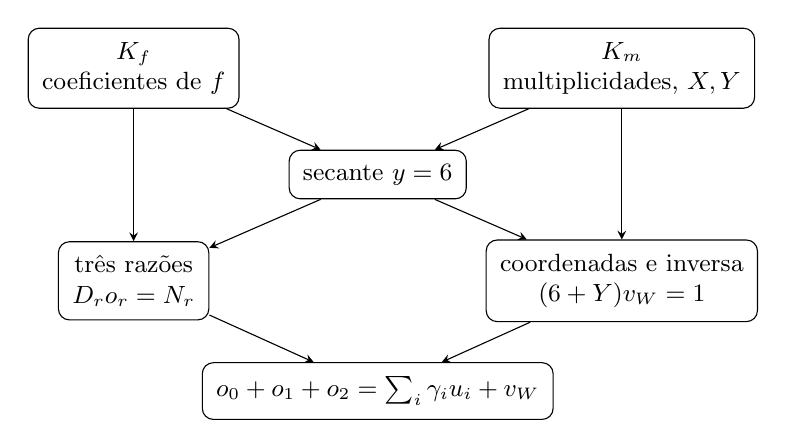
\begin{tikzpicture}[>=stealth,font=\small,
 box/.style={draw,rounded corners,align=center,inner sep=5pt}]
 \node[box] (kf) at (-3.1,0) {\(K_f\)\\coeficientes de \(f\)};
 \node[box] (km) at (3.1,0) {\(K_m\)\\multiplicidades, \(X,Y\)};
 \node[box] (line) at (0,-1.35) {secante \(y=6\)};
 \node[box] (fun) at (-3.1,-2.7) {três razões\\\(D_r o_r=N_r\)};
 \node[box] (point) at (3.1,-2.7) {coordenadas e inversa\\\((6+Y)v_W=1\)};
 \node[box] (sum) at (0,-4.1) {\(o_0+o_1+o_2=\sum_i\gamma_i u_i+v_W\)};
 \draw[->] (kf)--(line); \draw[->] (km)--(line);
 \draw[->] (kf)--(fun); \draw[->] (km)--(point);
 \draw[->] (line)--(fun); \draw[->] (line)--(point);
 \draw[->] (fun)--(sum); \draw[->] (point)--(sum);
\end{tikzpicture}
\end{center}

Temos agora os mesmos ingredientes da prova dos dois quadrados.
Naquela, duas portas e cinco linhas ligavam \(K,V\) ao resultado.
Nesta, as dezasseis linhas referem os dois compromissos vectoriais,
e o lado direito contém apenas constantes públicas. Assim, ao
formar o coeficiente reservado, Bob pode calcular todo o escalar
\(\delta+\langle\boldsymbol z,\boldsymbol b\rangle\) a partir
do circuito e dos desafios. Antes bastava-lhe um compromisso nesse
valor, porque a soma dos quadrados estava guardada em \(V\).
Agora a privacidade reside inteiramente nas duas listas e na
atribuição das portas. Os compromissos e as correcções da segunda
igualdade continuam indispensáveis para ligar o produto interno a
essas mesmas listas.

O exemplo pequeno tem uma vantagem precisa. Podemos acompanhar
cada linha da declaração e calcular os dois membros da igualdade final com os
mesmos dados que a demonstração manteve ocultos. Tem, também, a limitação natural do corpo
que escolhemos para ver os números. No limite probabilístico de
\eqref{eq:gbp-residuos}, dezasseis linhas e apenas dezasseis
desafios não nulos já dão a cota um. As igualdades acima estabelecem
a correcção dos cálculos da testemunha exibida. Para a solidez da
prova usam-se os parâmetros grandes, a vinculação a uma abertura e
as hipóteses de conhecimento estudadas com o protocolo
\cite{eagen-divisors,generalized-bulletproofs-fixed,monero-oxide-fcmp-source}.


Em FCMP++ a abertura oculta servirá para retirar a máscara de um ponto
e reconhecer esse ponto entre os filhos de um ramo. O verificador
conservará em cada passagem o que lhe é indispensável para a próxima,
a ligação ao mesmo compromisso.\hypertarget{excerto.generalizadas.fim}{}
